% !TeX program = pdflatex
\documentclass[tikz,border=8pt]{standalone}
\usepackage{pgfplots}
\pgfplotsset{compat=1.16}
\definecolor{FigureBlue}{HTML}{2563EB}
\definecolor{FigureOrange}{HTML}{EA580C}
\definecolor{FigureSlate}{HTML}{64748B}
\begin{document}
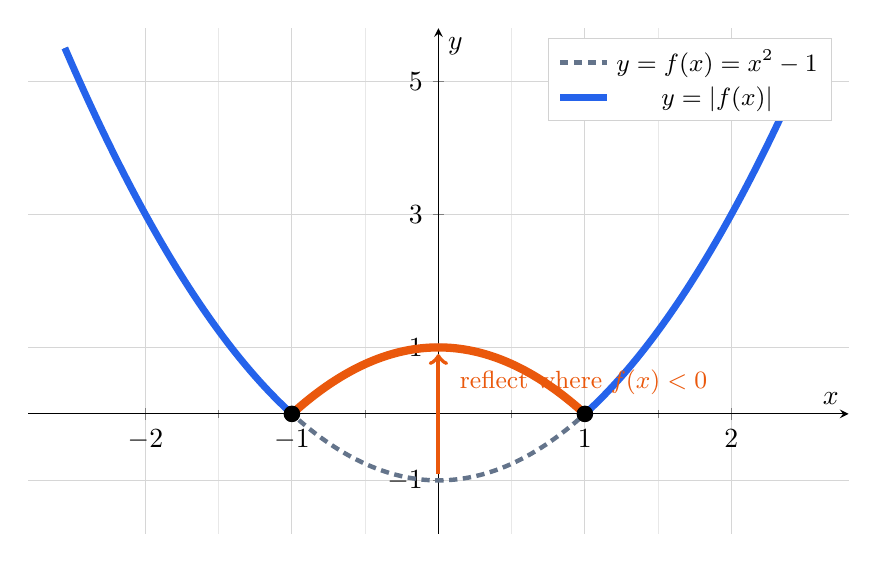
\begin{tikzpicture}
  \begin{axis}[
    width=12cm,height=8cm,axis lines=middle,
    xmin=-2.8,xmax=2.8,ymin=-1.8,ymax=5.8,
    xlabel={$x$},ylabel={$y$},xtick={-2,-1,0,1,2},ytick={-1,0,1,3,5},
    grid=both,minor tick num=1,grid style={draw=gray!18},major grid style={draw=gray!32},
    legend style={at={(0.98,0.98)},anchor=north east,draw=gray!35,fill=white,font=\small},clip=false,
  ]
    \addplot[FigureSlate,densely dashed,line width=1.6pt,domain=-2.55:2.55,samples=201] {x^2-1};
    \addlegendentry{$y=f(x)=x^2-1$}
    \addplot[FigureBlue,line width=2.5pt,domain=-2.55:2.55,samples=241] {abs(x^2-1)};
    \addlegendentry{$y=|f(x)|$}
    \addplot[FigureOrange,line width=3pt,domain=-1:1,samples=121] {1-x^2};
    \addplot[only marks,mark=*,mark size=2.8pt,black] coordinates {(-1,0) (1,0)};
    \draw[->,FigureOrange,line width=1.5pt] (axis cs:0,-.9) -- (axis cs:0,.9);
    \node[anchor=west,text=FigureOrange,font=\small] at (axis cs:.08,.48) {reflect where $f(x)<0$};
  \end{axis}
\end{tikzpicture}
\end{document}
